% !Mode:: "TeX:UTF-8"

\chapter{动态温度管理相关工作分析}


%温度不受管理将会给芯片带来严重的可靠性,性能,功耗和成本的问题。
%动态温度管理(DTM)技术就是用来解决这些问题,以控制芯片温度和功耗。

在这一章我们将介绍动态热管理相关的知识。首先 \ref{sec:adverse} 节将介绍芯片温度不受管理,处于高温状态或有高温点存在时,对芯片的可靠性,性能,功耗和散热成本不利影响。
 \ref{sec:DTM} 节将介绍具体的动态温度管理技术,包括动态电压频率调整、任务迁移等,详细分析其调整机制,和降低平衡芯片温度的原理。
 \ref{sec:pcm} 节介绍预测控制方法,仅仅有动态温度管理技术是不够的,这些技术需要有完整的引导控制才能发挥最大的作用,
 不进行合理的引导,不仅损害处理器性能,而且可能使处理器温度处于更加危险的地步。



\section{温度不受管理的影响}\label{sec:adverse}

因为我们持续减小芯片大小和要求高功耗下的性能,增长的芯片复杂性和功耗密度提高了芯片的峰值温度,也使温度梯度更加不均衡。
上升的峰值温度缩短芯片寿命,降低芯片性能,影响可靠性也增加散热成本~\cite{skadron:TACO'04}。上升的温度和静态功耗之间有正反馈的关系,有可能造成热失控。
在多核或者众核系统中,不同的应用负载或许引起核之间功耗和温度的不平衡。温度在时间和空间上的变化产生的芯片局部温度最大值叫做高温点~\cite{Donald:ISCA'06}。
过多的空间上的温度差也就是热梯度增加时钟抖动降低性能和可靠性。
上升的温度需要更多的散热能力去冷却处理器,一个典型的散热风扇会消耗高达服务器 $51\%$ 的功耗~\cite{lefurgy2003energy,ayoub2010gentlecool}。

\subsection{温度对系统可靠性的影响}\label{sec:reliability}
高功耗的一个最明显的结果就是上升的芯片温度,高温对芯片最严重的的后果就是损害芯片的可靠性。在高温状态下,载流子迁移率降低,会导致当代 CMOS 技术下的器件变慢。
而且还可能导致器件失效,下面是温度相关的半导体器件失效机理~\cite{jedec2003failure}:
%\begin{itemize}
%\item 电迁移(EM):(查的失效机理)由于传导电子和扩散金属原子之间的动量交换,金属线中例子会逐步移动,这样会导致金属线形变。甚至会引起金属线断开导致器件失效。
%\item 应力迁移(SM):金属原子在机械应力梯度下会发生移动导致金属线变形。不同材料的热膨胀率不同会产生应力。这个也会引起金属线断开导致器件失效。
%\item 介质击穿(DB):当介质中形成一个导电通路,电路的阴阳极短路时,介质失效。
%\end{itemize}
\begin{description}
\item[电迁移($EM$) :] ~由于传导电子和扩散金属原子之间的动量交换,金属线中离子会逐步移动,这样会导致金属线形变。它甚至会引起金属线断开导致器件失效。
\item[应力迁移($SM$) :] ~金属原子在机械应力梯度下会发生移动导致金属线变形。不同材料的热膨胀率不同会产生应力。这个也会引起金属线断开导致器件失效。
\item[介质击穿($DB$) :] ~当介质中形成一个导电通路,电路的阴阳极短路时,介质失效。
\end{description}

这些机理引起的失效时间($TF$)可以被表示为下式:
\begin{equation}
TF = A \cdot e^{E_a/(k \cdot T)}
\end{equation}
其中$A$ 是一个常数,$E_a$ 活化能量(eV),$k$ 是玻尔兹曼常数($8.62 \times 10^{-5}$ eV/K)。
这些都是正常数, $T$ 是器件的操作温度(K)。
所以, $TF$ 是温度的递减函数。
当温度上升时, $TF$ 会指数下降。这就意味着器件将极快速失效。

互连电阻率也随温度升高而升高,会引起更长的互连 RC 延迟,导致性能损失和时序噪声分析复杂化。
高温环境还严重缩短互连和器件的寿命。

温度高不是系统可靠性问题的唯一原因。另外还有两个热现象即热循环和热梯度也会严重影响器件的可靠性。
热循环是操作温度的暂时波动,可能是由器件的正常功率上升或者下降引起。
另外也可能因为任务负载的变化或者设备的功耗管理策略,比如设备的部件在几种功耗模式下很频繁的切换。
热循环可以会削弱材料,引起介质裂开或者焊料疲劳等的不同失效。
热循环的失效率可以表示为:
\begin{equation}
\lambda \propto \Delta T^q
\end{equation}
其中 $\Delta T$ 是热循环的幅度,$q$ 是热循环的频率。
温度波动越大或者越频繁,器件失效率就越大。

热梯度是整个芯片温度在空间上的不平衡,热梯度和局部高温点严重影响封装可靠性。
因为现在片上系统(SoC)和多核众核芯片上负载不均衡,这样温度就会不平衡,引起大的温度梯度。
大的温度梯度最重要的影响是互连电阻不均衡,这会导致时钟偏差。这个是同步数字电路中很不希望发生的,会引起时序冲突。

\subsection{温度对静态功耗的影响}\label{sec:leakage}

温度不仅是功耗的结果,在某种程度上功耗和温度互为因果。
这是因为,静态功耗很大程度上取决于操作温度。当前静态功耗已经是系统总功耗的很明显的一部分,而且会随技术继续增长。
温度和静态功耗之间的关系已经被广泛的研究过~\cite{liao2005temperature},漏电流可以表示为:
\begin{equation}
I_{leak} = I_s \cdot A \cdot T^2e^{\frac{\alpha + \beta V_{dd}}{T}}+B
\end{equation}
其中, 对于指定的技术, $A$ 、 $B$ 、  $\alpha$ 、 $\beta$ 是温度无关的正常数。
$V_{dd}$ 是供电电压,$I_s$ 是在指定温度和供电电压下的基准漏电流。
我们可以看出温度对漏电流的影响是 $T^2e^{1/T}$ 。图~\ref{fig:leakage}是漏电流对温度的曲线。
\begin{figure}
  \centering
    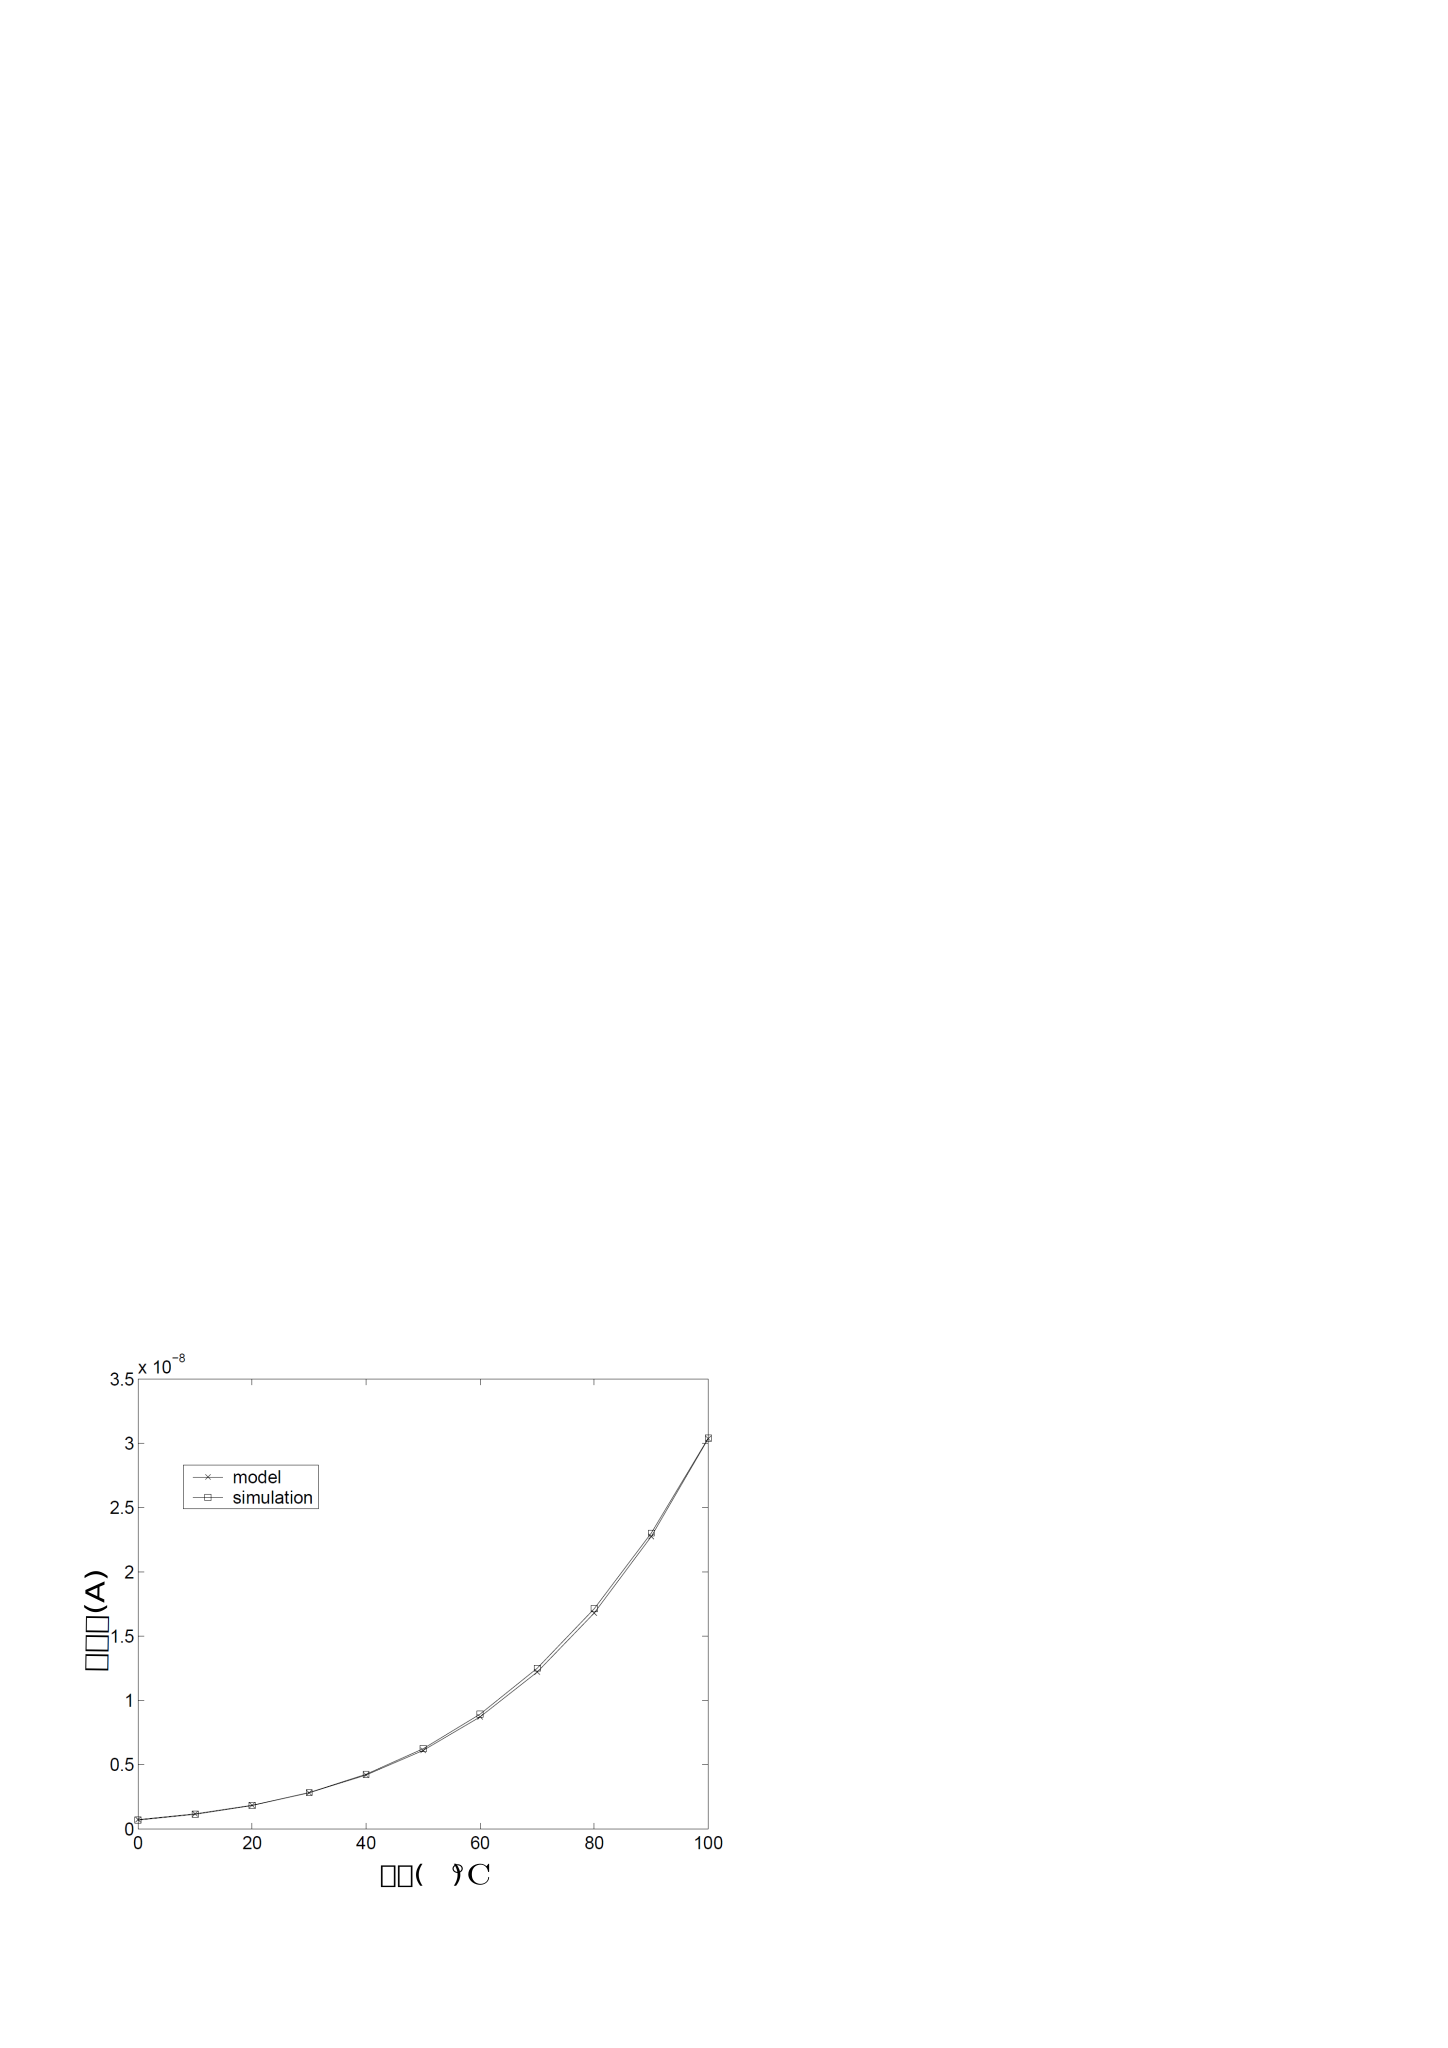
\includegraphics[width=0.7\columnwidth]{fig/leakage}
  \caption{温度与漏电流的关系\cite{zhang2003hotleakage}}\label{fig:leakage}
\end{figure}

\subsection{温度对冷却系统的影响}\label{sec:cooling}

上升的温度另一个明显的坏处就是冷却成本变得更高。
为了保证芯片正常运行,芯片不得不配备成本更高的封装来散热。
对于常规散热风扇型的冷却方法,散热风扇不得不在一个更高的速度上运行来散去芯片产生的额外的热量。
这是因为散热器的散热能力是由热阻$R_{h2a}$ (h2a表示从散热器到外部环境)决定,热阻$R_{h2a}$又是由散热风扇速度决定的,如下式:
\begin{equation}\label{eq:cooling}
R_{h2a} = (h_1v_f(1-e^{\frac{h_2v_f^{h_3}+h_4}{h_1v_f}}))^{-1}
\end{equation}

在式\eqref{eq:cooling}中,$h_1$ 、 $h_2$ 、 $h_3$ 、 $h_4$是芯片的特定物理系数,$v_f$ 是散热风扇速度。
风扇功耗 $P_{fan}$正比于风扇转速的立方,即 $P_{fan} \propto v_f^3$。
这意味着高的温度不仅是风扇功耗上升,同时也降低了风扇的使用寿命。

\section{动态温度管理相关技术}\label{sec:DTM}

前面已经说明,温度不受管理将会带来严重的可靠性,性能,功耗和成本的问题。
为应对热问题,这方面的研究已经很多,静态热管理技术也很早被研究过。
比如,热感知的版图布局规划。
在设计阶段将芯片的最热的功能单元之间留出空间,以便该单元的热量能更多地散热到周围。
更进一步的布局规划是通过独特的布局规划将这些功能单元分解成更小的组成部分。
但是这种方法并不适用于现在更加广泛复杂的应用。
动态温度管理(DTM)技术就是用来解决上述问题,来控制芯片温度和功耗。
随着温度被调整,系统的可靠性就可以提升。适当的降低电子设备的温度 $10^{\circ}$C $\sim 15^{\circ}$C 可以使设备寿命延长两倍。
对于金属结构,热循环幅度减少 $10^{\circ}$C 可以使平均失效时间增长16倍。
温度降低时静态功耗也会显著减少~\cite{kursun2006investigating}。温度每降低 $9^{\circ}$C ,静态功耗降低 50\%~\cite{liu2007accurate} 。
这对于将来的片上系统设计非常重要。因为静态功耗估计将会超过总功耗的 50\% 。
调控温度不仅能保证芯片可靠性和降低静态功耗,而且还能提升性能。在低温时,晶体管的开关速度更快~\cite{pamula2003cooling} 。
平衡的空间热梯度可以显著减轻时钟偏移问题。

动态温度管理需要能使芯片自主修改任务的执行和功耗特性的技术,以使低开销的冷却方法也能保证芯片在安全温度以内。
动态温度管理控制器在系统运行时监控系统信息,并采取相应的热管理措施。以最小的性能损耗,尽可能地把系统温度保持在安全阈值以下,尽量平滑地修正热分布。

对一个计算系统执行动态热管理,需要的最重要的系统信息是芯片温度。这个信息可以从片上温度传感器的到,或者用热模型估计。
一些最先进的动态温度管理技术还需要温度信息,应用程序特性,任务功耗等等。

\subsection{动态温度管理和动态功耗管理的不同}\label{sec:DPM}

尽管温度基本上是由功耗引起的,动态温度管理也需要修正功耗特性,甚至动态功耗管理和动态温度管理都用相同的措施想动态电压频率调整(DVFS)和任务迁移,
但是在动态功耗管理和动态温度管理上有几个明显的不同点。
首先,系统温度分布不仅仅只跟功耗分布相关。因为功耗可以瞬间改变,但是温度是功耗的的积累,在时间和空间上改变都很慢。
打个比方,功耗就像 RC 电路中的电流源,温度就像各个节点的电压。
所以温度的行为就像一个低通滤波器,滤掉了功耗变化中的高频部分。
第二,温度正比于功耗密度 , $ T \propto P/A$,这里 $A$ 是面积。
所以即使不能降低功耗,我们可以分配功耗到更大的面积上,这样仍然可以降低温度。
比如所有进程都合并在一个核上,芯片上这一小部分的负载很重,最好从散热的角度将他们分配到多个核上。
第三,比起温度管理策略,功耗管理策略可能有冲突的目标,有产生不期望的温度分布的可能。
比如,功耗管理策略可能为了节省功耗非常频繁的将器件切换到低功耗状态。
\ref{sec:reliability}节中提到过这个调整会产生大幅度和频繁的热循环,加速封装疲劳。
为了实现低功耗,功耗管理策略可能关掉一些部件整合计算,这会产生局部高温点和大的温度梯度。
\\
\begin{figure}
  \centering
    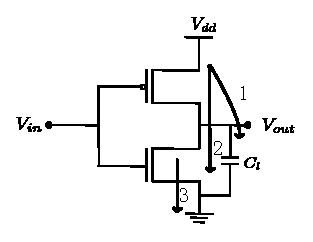
\includegraphics[width=0.7\columnwidth]{fig/inverter}
  \caption{简单CMOS反相器功耗示意图}\label{fig:inverter}
\end{figure}

\subsection{动态电压频率调整技术}\label{sec:DVFS}

过去 动态电压频率调整技术(DVFS)被广泛应用于功耗和能量优化中,随着芯片热问题的凸显,DVFS 也被广泛应用在处理器热管理中。
DVFS 成为一种被广泛应用的动态温度管理技术。DVFS 技术是调整处理器的时钟频率和电源电压,当处理器时钟频率降低时,电源电压也可以相应地降低。
这样可以降低功耗,甚至于节省能量~\cite{le2010dynamic}。
DVFS 技术在计算系统中应用广泛,从嵌入式,到平板,桌面系统,以至于到高性能服务器系统。

现在大多数数字电路都是 CMOS 电路,尤其是在处理器方面。所以我们简要分析一下 CMOS 电路的功耗,找出功率,电压,频率之间的关系。
CMOS 电路的功耗是动态功耗,静态功耗和电路短路功耗的综合,这些功耗如图~\ref{fig:inverter}所示:
\begin{itemize}
\item  ~$P_d$ 表示动态功耗,源于电容的充电和放电(1)。
\item  ~$P_s$ 表示静态功耗,源于晶体管反向偏置(2)。
\item  ~$P_{sh}$ 表示电路短路电流,源于开关时 $V_{dd}$ 到 $GND$ 的直接通路(3)。
\end{itemize}
CMOS电路总功耗表示为:
\begin{equation}\label{eq:cmos}
P_{cmos} = P_d + P_s + P_{sh} 
\end{equation}


动态功耗是 CMOS 电路功耗的很大一部分,\ref{sec:leakage}中已经提到近年来静态功耗也占据总功耗的很大一部分,其可以表示如下:
\begin{equation}\label{eq:DVFS}
\begin{split}
P_d &= CfV_{dd}^2 \\
P_s &= I_lV_{dd}  
\end{split}
\end{equation}
其中,  $C$ 是晶体管栅极电容(取决于它的特征尺寸),
$f$ 是操作频率,$V_{dd}$ 是电源电压, $I_l$ 为漏电流。

动态电压频率调整技术降低电压可以有效地减少功耗。
动态功耗可以显著减少,因为上面显示 $P_d \propto V^2$ 。静态功耗也可以减少。
 降低电源电压会限制操作频率~\cite{suleiman2005dynamic},其关系可表示为:
 \begin{equation}\label{eq:fv}
 f \propto \frac{(V_{dd} - V_t)^2}{V_{dd}} 
 \end{equation}
 其中 $V_t$ 表示 CMOS 阈值电压。这也就是说,频率的降低可以伴随着电压也做降低调整。
 时钟频率 $f$ 降低一半时,能降低处理器功耗,任务完成时间会延长,但是总的能量并没有少。程序运行时间增加会显著影响处理器性能,这也是 DVFS 的缺点之一。
 当电源电压也降低一半时,功耗将会继续降低,但是任务完成时间并没有继续延长,这样能量也被减少了。如图~\ref{fig:energy}所示。
 
\begin{pics}{任务的功耗与能耗}{fig:energy}
\addsubpic{最大电压频率运行时的功耗与能耗}{width=0.5\columnwidth}{fig/energy1}
\addsubpic{频率减半时的功耗与能耗}{width=0.5\columnwidth}{fig/energy2}
\addsubpic{电压频率都减半时的功耗与能耗}{width=0.5\columnwidth}{fig/energy3}
\end{pics}

为了在多频处理器上执行 DVFS 操作,操作系统需要先预测或者估计将来的任务负载(比如通过 MPC 方法,后面会介绍),然后将其转换为频率值 $f_{des}$。
这个值被用于调整处理器的时钟频率 $f$  和 电源电压 $V_{dd}$。 
~\cite{Zanini:ECCTD'09} 中的方法就是用 MPC 方法做预测,用 DVFS 做调整,保证芯片在安全温度以下。
因为DVFS通过降低处理器的操作频率来降低功耗会增加程序运行时间,这会显著影响处理器性能。
所以很多方法中 DVFS 并不是单独使用,往往结合任务迁移来降低对处理器性能的影响(下面将详细介绍任务迁移)。

\subsection{任务迁移技术}\label{sec:taskm}

对于多核或者众核处理器来说,每个核运行不同的任务,或者每个核上的任务数量不同。
这样的话核与核之间的负载不同,各核的功耗不同,导致温度不平衡。
其实即使负载功耗相同,各核的散热参数也不同,也会导致温度不平衡。这对多核处理器还不明显,因为核数少各核的散热参数基本相同,
但是对于众核处理器这就是一个很明显的问题了。 在 \ref{sec:adverse} 中已经说明温度梯度会严重影响芯片的可靠性,静态功耗等。
所以解决温度不平衡非常关键,任务迁移是一个很好的解决方法。

任务迁移是任务管理的一种特殊形式,就是将任务从一个计算环境迁移到另一个计算环境中。
这本来是一种用在分布式计算中的技术,但现在随着多核众核处理器的出现,其应用更加广泛了。
在多核处理器中,任务迁移是任务调度的一个标准部分,它的过程很简单,就是将一个任务从一个核迁移到另个核上去运行。

下面介绍一个例子来说明任务迁移,如图 \ref{fig/TM} 。
双核处理器上运行着三个任务(A、B、C),每个核可以独立设置其时钟频率和电源电压来降低功耗,去满足当前负载的需求。
任务负载由全速等效负载(FSE)表示,全速等效负载是一个任务在核上以最大频率运行时的负载。
核 1 上运行任务 A 和 B ,分别有 $ 50\% $ 和 $ 40\%$ 的等效 FSE ;
核 2 上运行任务 C ,有 $ 40\%$ 的等效 FSE 。
在这个例子中,核 1 在理想状态下,可以将频率调整为最大频率的 $90\%$ ,核 2 可以将频率调整为最大频率的 $40\%$。
这样是最能减少功耗的。但是这样仅仅用 DVFS 方法并不能平衡芯片的温度。
在这个例子中,因为负载不同,核 1 的温度将会高于 核 2。
因此,处于对温度平衡的考虑,可以将任务 B 在两个核上周期地迁移。
这样两个核的负载就会平均($ 40\% + 50\% = 65\% $)。
这是一个双核简单任务迁移的例子。对于更多核的处理器,任务迁移策略不会这么简单,需要由理论上的算法去计算如何迁移。
\pic{简单的任务迁移例子~\cite{mulas2008thermal}}{width=0.7\columnwidth}{fig/TM}


\section{预测控制方法}\label{sec:pcm}

上面介绍了动态温度管理技术,然而这些技术是实际的操作。
如果只应用这些技术,依靠温度传感器的温度数据,是无法避免高温事件的。因为那只能在超过安全阈值之后才能采取操作,动态温度管理操作严重延时。
这样不仅管理效果不好,而且还可能引起更大的问题,比如某核上任务负载较小温度较低,将要将其与高温核上任务交换。但是延时之后该任务负载加重,这样就会使高温核上出现更高的温度。
针对这问题,对动态温度管理技术提供指导性调整意见就很重要了。
这里我们介绍一些预测控制方法。
\subsection{芯片温度预测方法}\label{sec:temperature}
对于预测控制,最简单的就是预测温度。温度预测技术是控制决策的基础,只要预测是准确的,提前才去适当的操作就可以避免高温事件。
温度预测技术方面的研究已经很多,过去常用的温度预测控制方法是,直接对将来芯片的温度,和负载功耗进行预测。根据预测出的下一时刻的温度,反过来对现有的负载功耗进行调整。
这里我们简要介绍两种温度预测方法,它们的主要区别是温度预测模型不同,
基于递归最小二乘法(RLS)的温度预测~\cite{yeo2008predictive} 和基于自回归移动平均值(ARMA)的温度预测~\cite{coskun2008proactive} 。

在~\cite{yeo2008predictive}中,通过分析,影响芯片温度变化快慢有两个因素,一个是当前温度与稳态温度的差值,另一个是应用程序本身。
第一个因素是长期的温度行为,第二个因素是短期的温度行为。基于这个分析,基于 RLS 的温度预测由两部分组成:基于应用程序的温度模型(ABTM)做短期温度预测,
基于核的温度模型(CBTM)做长期温度预测。 ABTM 通过观察应用程序近期的温度行为,然后将这一信息纳入递归最小二乘回归模型来预测将来的温度,如式 \eqref{eq:RLS} 所示。
\begin{equation}\label{eq:RLS}
y = \theta_1u_1 + \theta_2u_2 + \cdots + \theta_nu_n
\end{equation}
其中, $y$ 是将要预测的温度, $u_i$ 是最近的 $n$ 个时刻的温度,$\theta_i$ 是 RLS 模型将要估计的系数。 CBTM 模型考虑核的长期热行为。
它忽略应用的短期功耗变化,假设应用在一个稳定的功耗运行。 CBTM 的温度变化公式如式 \eqref{eq:CBTM} 所示。
\begin{equation}\label{eq:CBTM}
T(t) = T_{ss} -(T_{ss} - T_{init}) \times e^{-bt}
\end{equation}
其中,$T_{ss}$ 是稳态温度, $T_{init}$ 是初始温度, $b$ 是温度常数。$T_{ss}$ 对每个应用是预先计算的,  
$b$ 是线下计算的,由芯片热特性觉定,所以对所有只需要计算一次。用式 \eqref{eq:CBTM} 就可以预测时间 $t$ 之后的处理器温度。
这样就得到了两个预测的温度,最终的温度预测是这两个温度的权重和,如式 \eqref{eq:wsum}所示。
\begin{equation}\label{eq:wsum}
T_{predict} = w_sT_{ABTM} + w_lT_{CBTM}
\end{equation}
这样芯片将来的温度就可以预测,根据这个温度,来做动态温度管理操作,将芯片温度控制在安全温度以下。这就是~\cite{yeo2008predictive}的温度预测控制方法。

在~\cite{coskun2008proactive}中,  ARMA 预测模型的原理是,当负载不变时,通过回归过去的测量,可以准确地估计温度。
式  \eqref{eq:ARMA} 就是 ARMA 模型, 这与RLS模型相似,因为他们都是基于线性回归的模型。
\begin{equation}\label{eq:ARMA}
y_t + \sum_{i=1}^qa_iy_{t-i} = e_t +\sum_{i=1}^qc_ie_{t-i}
\end{equation}
其中,$y_t$ 是时刻 $t$ 的温度, $e_i$ 叫做预测误差或者残留噪声。与 RLS 模型相似,系数 $a_i$ 和 $c_i$ 是 ARMA 模型通过计算确定的。
该方法也是根据预测的温度来进行动态温度管理操作。

但是通过这两种温度预测控制方法,我们可以看出,即使温度的预测是准确,也并不能对动态温度管理操作提供指导性意见。
比如我们要采用 DVFS 操作降低功耗来降低温度,但是我们并不知道将电压和频率降低到什么水平才合适。 
假如采用任务迁移方法,我们也并不知道具体多大功耗的任务适合迁移到最低温度的核上,因为高功耗任务迁移到低温核上可能引起更高的高温点。

\subsection{模型预测控制方法}\label{sec:mpc}
%\begin{figure}
%  \centering
%    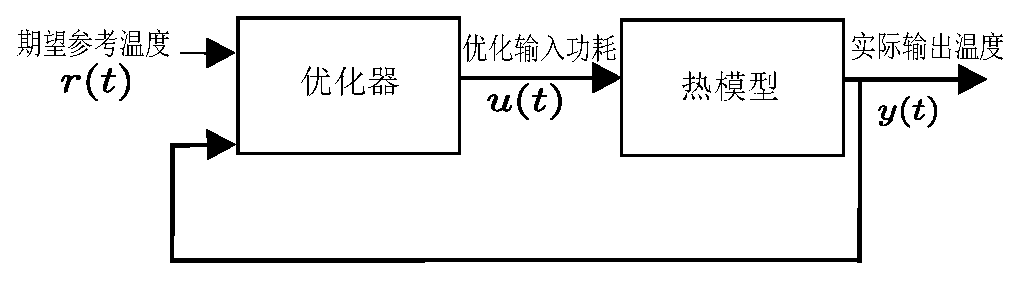
\includegraphics[width=0.7\columnwidth]{fig/mpcshow}
%  \caption{模型预测控制基本结构}\label{fig:mpcshow}
%\end{figure}
\pic{模型预测控制基本结构}{width=0.7\columnwidth}{fig/mpcshow}

最近,针对 \ref{sec:temperature} 节中的问题,即仅仅预测温度并不能很好的给动态温度管理操作提供很好的指导性意见,
模型预测控制(MPC)方法~\cite{Wang:MPC_BOOK'09} 被引入到动态温度管理中~\cite{Zanini:ECCTD'09},该方法可以给动态温度管理操作提供良好的指导性意见。
下面我们介绍一下模型预测控制方法。

图~\ref{fig/mpcshow}是模型预测控制方法的概念结构。 MPC 用在动态温度管理中源于这样的想法,采用用于控制处理器的热模型做预测,预测给定期望温度下的所需的功耗。
注意,该预测方法与 \ref{sec:temperature} 节中的温度预测方法不同, MPC 并不是预测温度,而是根据设定的温度和处理器的热模型来预测输入功耗为多大。
这种预测能力允许在线解决优化控制问题,在未来的预测时间内,对应的优化输入和输出可以使跟踪误差最小化。 跟踪误差就是期望的温度和预测的温度的差值。

优化的结果根据滚动优化策略来采用~\cite{bemporad1999robust},如图~\ref{fig/mpc}所示。$N_p$ 表示预测范围或者输出范围长度,$N_m$ 表示控制范围或者输入范围长度。
在时刻 $t$ 进行预测时,设定$N_p$ 长度范围的期望输出温度,即图中虚线所示。这样就可以预测出可以操纵的输入功耗 $u$ 和预测出的输出温度 $y$ 。
在预测出的优化输入功耗序列($ u(t) $ 到 $ u(t+N_m-1) $)中,只应用第一个 $ u(t)$ 。优化序列中的其余值被丢弃,在时刻 $t+1$ 进行新一轮的预测。这就是滚动优化策略。 
%\begin{figure}
%  \centering
%    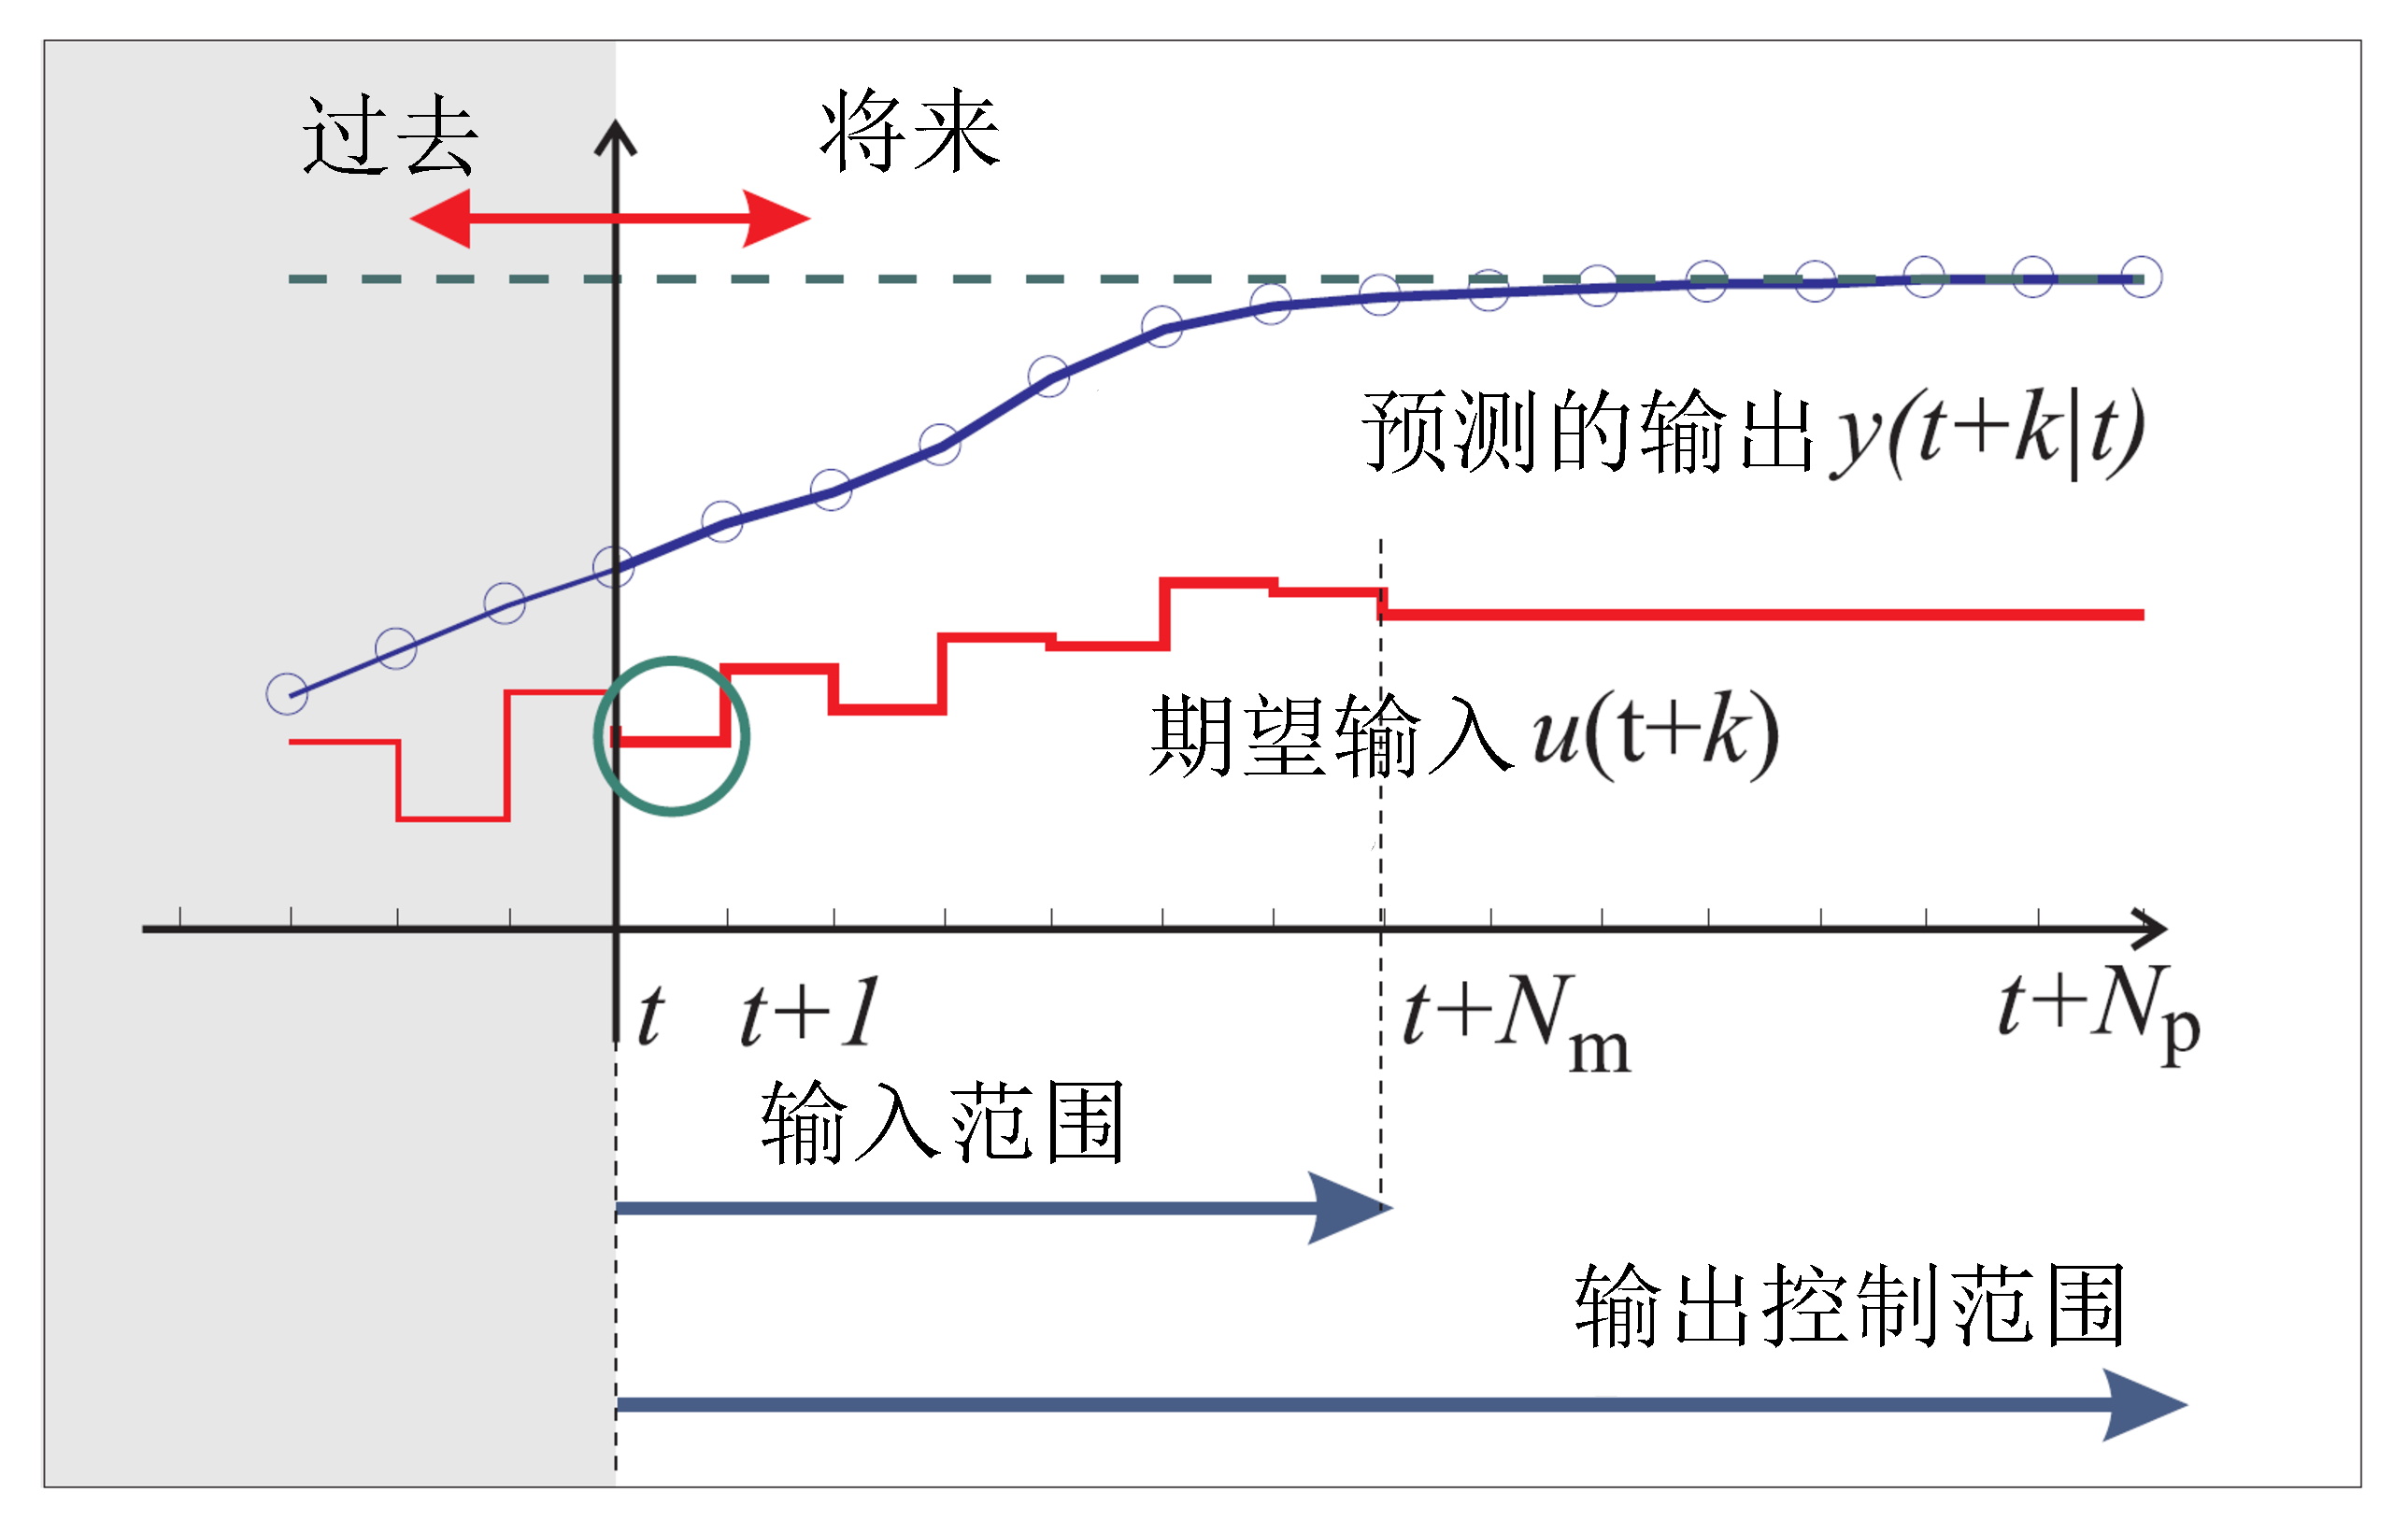
\includegraphics[width=0.7\columnwidth]{fig/mpc}
%  \caption{滚动优化策略(只有预测得到的第一步$u$被采用)~\cite{bemporad1999robust}}\label{fig:mpc}
%\end{figure}
\pic{滚动优化策略(只有预测得到的第一步$u$被采用)~\cite{bemporad1999robust}}{width=0.7\columnwidth}{fig/mpc}



\section{本章小结}\label{sec:xiaojie2}

本章首先分析了温度不受管理的情况下,会严重影响芯片可靠性,寿命和性能。高温对功耗也有互为因果的关系。对于常规散热片,散热成本也是急剧增加。
然后,对动态温度管理相关技术进行介绍,详细分析动态电压频率调整技术通过调整电压频率对功耗的影响。对任务迁移技术也进行详细说明。
动态热管理技术需要好的控制方法做引导,最后介绍温度预测方法和模型预测控制方法,完整的引导控制策略才能让动态热管理技术发挥最大作用。
本论文的方法就是将模型预测控制方法与电压频率调整技术和任务迁移技术相结合。























%我们已经进入众核处理器时代\cite{MaWang:APCCAS'14}.
%2012年,英特尔正式将第一代集成众核产品,代号为Knights Corner的协处理器推向市场。
%这一代产品使用P54C核心构建,片上集成61个CPU核心,实现了GPU级别的浮点运算速度。
%英特尔至强披™协处理器X100系列(代号为“Knights Corner”)是第一代英特尔®集成众核(英特尔®MIC)架构,
%它结合了许多英特尔的CPU内核在单一芯片上的。
%该生产线是针对高度并行的工作负载在各种领域,如计算物理,化学,生物和金融服务。
%Knights Corner片上集成了高达61核心。